\documentclass{article}

\usepackage{amsmath, wrapfig}

\usepackage{tikz}
\usetikzlibrary{calc}

\begin{document}

\pagenumbering{gobble}

\begin{wrapfigure}{l}{0.3\linewidth}
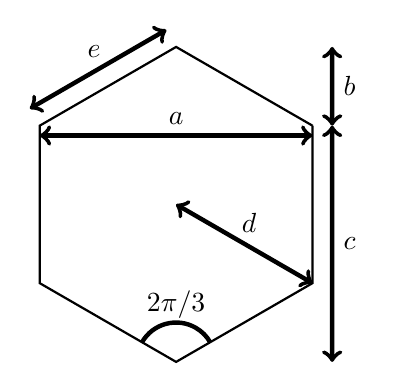
\begin{tikzpicture}
% cell centre
\coordinate (A) at (0, 0);
% cell corners
\coordinate (B) at ($(A) + ({2*cos(30 + 0*60)}, {2*sin(30 + 0*60)})$);
\coordinate (C) at ($(A) + ({2*cos(30 + 1*60)}, {2*sin(30 + 1*60)})$);
\coordinate (D) at ($(A) + ({2*cos(30 + 2*60)}, {2*sin(30 + 2*60)})$);
\coordinate (E) at ($(A) + ({2*cos(30 + 3*60)}, {2*sin(30 + 3*60)})$);
\coordinate (F) at ($(A) + ({2*cos(30 + 4*60)}, {2*sin(30 + 4*60)})$);
\coordinate (G) at ($(A) + ({2*cos(30 + 5*60)}, {2*sin(30 + 5*60)})$);
% junctions
\draw[thick] (B) -- (C) -- (D) -- (E) -- (F) -- (G) -- (B);
% lengths
\coordinate (H) at ($(D) + ({0.25*cos(120)}, {0.25*sin(120)})$);
\coordinate (I) at ($(C) + ({0.25*cos(120)}, {0.25*sin(120)})$);
\draw[<->, ultra thick] (H) -- (I) node[midway, above left, xshift=5pt]{$e$};
\coordinate (J) at ($(D) + (0, -0.125)$);
\coordinate (K) at ($(B) + (0, -0.125)$);
\draw[<->, ultra thick] (J) -- (K) node[midway, above]{$a$};
\coordinate (L) at ($(B) + (0.25, 0)$);
\coordinate (M) at ($(C) + ({sqrt(3) + 0.25}, 0)$);
\draw[<->, ultra thick] (L) -- (M) node[midway, right]{$b$};
\coordinate (N) at ($(F) + ({sqrt(3) + 0.25}, 0)$);
\draw[<->, ultra thick] (L) -- (N) node[midway, right]{$c$};
\draw[<->, ultra thick] (A) -- (G) node[midway, above right, xshift=-5pt]{$d$};
% angles
\draw[ultra thick] ($(F) + ({0.5*cos(150)}, {0.5*sin(150)})$) arc(150:30:0.5) node[midway, above, yshift=-2.5pt]{$2\pi/3$};
\end{tikzpicture}
\end{wrapfigure} 

\begin{align}
a &= 2 e \cos\left(\frac{\pi - 2\pi/3}{2}\right) = \sqrt{3} e\\
b &= e \sin\left(\frac{\pi - 2\pi/3}{2}\right) = \frac{1}{2} e\\
\left(\frac{a}{2}\right)^2 + b^2 &= e^2\\
c &= b + e = \frac{3}{2} e\\
d &= \frac{e/2}{\cos(\pi/3)} = e\\
\mathrm{Area} &= 6 \left[\frac{1}{2} e \frac{a}{2}\right] = \frac{3\sqrt{3}}{2} e^2\\
e &= \sqrt{\frac{2 \mathrm{Area}}{3 \sqrt{3}}}
\end{align}

\end{document}

